%%%%%%%%%%%%%%%%%%%%%%%%%%%%%%%%%%%%%%%%%%%%%%%%%%%%%%%%%%%%%%%%%%%%%%%%%%%%
%% Author template for Syngenta Crop Challenge (syngen)
%% -- based on Author template for Operations Research (informs3.cls)
%%%%%%%%%%%%%%%%%%%%%%%%%%%%%%%%%%%%%%%%%%%%%%%%%%%%%%%%%%%%%%%%%%%%%%%%%%%%
\documentclass[syngen,nonblindrev]{informs3-syngen} 

\DoubleSpacedXI % Made default 4/4/2014 at request
%%\OneAndAHalfSpacedXI % current default line spacing
%%\OneAndAHalfSpacedXII
%%\DoubleSpacedXII

\usepackage{endnotes}
\let\footnote=\endnote
\let\enotesize=\normalsize
\def\notesname{Endnotes}%
\def\makeenmark{$^{\theenmark}$}
\def\enoteformat{\rightskip0pt\leftskip0pt\parindent=1.75em
  \leavevmode\llap{\theenmark.\enskip}}

% Private macros here (check that there is no clash with the style)

% Natbib setup for author-year style
\usepackage{natbib}
 \bibpunct[, ]{(}{)}{,}{a}{}{,}%
 \def\bibfont{\small}%
 \def\bibsep{\smallskipamount}%
 \def\bibhang{24pt}%
 \def\newblock{\ }%
 \def\BIBand{and}%

%% Setup of theorem styles. Outcomment only one.
%% Preferred default is the first option.
\TheoremsNumberedThrough     % Preferred (Theorem 1, Lemma 1, Theorem 2)
%\TheoremsNumberedByChapter  % (Theorem 1.1, Lema 1.1, Theorem 1.2)
\ECRepeatTheorems

%% Setup of the equation numbering system. Outcomment only one.
%% Preferred default is the first option.
\EquationsNumberedThrough    % Default: (1), (2), ...
%\EquationsNumberedBySection % (1.1), (1.2), ...


%%%%%%%%%%%%%%%%
\begin{document}
%%%%%%%%%%%%%%%%

% Corresponding author's name for the running heads
\RUNAUTHOR{Xavier Ignacio Gonzalez}

% Title or shortened title suitable for running heads. Sample:
% \RUNTITLE{Bundling Information Goods of Decreasing Value}
% Enter the (shortened) title:
\RUNTITLE{Robust Decision Making in Soybean Seed Variety Selection}

% Full title. Sample:
% \TITLE{Bundling Information Goods of Decreasing Value}
% Enter the full title:
\TITLE{Robust Decision Making in Soybean Variety Selection}

% Corresponding author or team lead. A single point of contact for each team submission is requested. 
\ARTICLEAUTHORS{%
\AUTHOR{Xavier Ignacio Gonzalez}
\AFF{542 West 112\textsuperscript{th} Street 8E, New York City, NY, 10025, United States, \EMAIL{xig2000@columbia.edu}} %, \URL{}}
} % end of the block

\ABSTRACT{%
A novel alternative approach to support soybean seed variety selection decision is presented in this study. 
The implementation of Robust Decision Making (RDM) is suitable for this purpose because it allows farmers to deal with the deep uncertainty about the climate conditions and mitigate the risks of a low outcome. 
By exploring the scenario space using machine learning technics, RDM suggests robust strategies, rather than optimal, which are those strategies that perform acceptable well over a wide range of scenarios. 
This research discusses in detail the procedure to implement said methodology. 
It starts describing the pre-processing of the data, a clustering to group observations, and a Principal Components Analysis to improve the pattern recognition.
Then, varieties V41 and V187 are identified as possible candidates of robust strategies. 
Exploring the space by classification tree algorithm, this study reveals possible vulnerabilities for the candidates in the evaluated site: V41 returns low values of yield when average temperatures are low, and V187 is not a good choice depending on the distribution of rainfalls.
A mix that contains (i) 60\% of V41, (ii) 30\% of V98, and (iii) 10\% of V180 is identified as a possible robust strategy as it limits those risks detected.

% Enter your abstract
}%

% Fill in data. If unknown, outcomment the field
\KEYWORDS{Robust Decision Making, Decision Tree, Scenario Planning, Crop Mix Allocation, Farm Planning, Clustering, Principal Component Analysis}

\maketitle
%%%%%%%%%%%%%%%%%%%%%%%%%%%%%%%%%%%%%%%%%%%%%%%%%%%%%%%%%%%%%%%%%%%%%%

% Samples of sectioning (and labeling) 
% NOTE: (1) \section and \subsection do NOT end with a period
%       (2) \subsubsection and lower need end punctuation
%       (3) capitalization is as shown (title style).
%
%\section{Introduction.}\label{intro} %%1.
%\subsection{Duality and the Classical EOQ Problem.}\label{class-EOQ} %% 1.1.
%\subsection{Outline.}\label{outline1} %% 1.2.
%\subsubsection{Cyclic Schedules for the General Deterministic SMDP.}
%  \label{cyclic-schedules} %% 1.2.1
%\section{Problem Description.}\label{problemdescription} %% 2.

% Text of your paper here

\section{Introduction}
One major way in which decision-makers can adapt to a shifting context (e.g., climate conditions) in agriculture is by changing the allocation of land among a set of viable activities (e.g., different seed varieties), the same way an investor re-balances a stock portfolio as markets change. 
Traditionally, the land allocation decision follows a predict-then-act process where the farmers require an accurate, and increasingly precise, assessment of the future impacts of climate in order to adapt successfully. 
See for instance \cite{messina1999land}.
Although deliberative decision support mechanisms (e.g., optimization of an objective function or metric) have a strong tradition in agricultural economics, they often have been dismissed as unrealistic as they do not model accurately all uncertainties involved, see \cite{rivera2011recognising}. \par
In this study, a novel approach to address this difficulty is presented. 
Some ideas are taken from robust decision-making methodology (RDM) introduced in \cite{lempert2003shaping} to examine the performance of different soybean variety allocation mixes over a range of plausible scenarios driven by uncertainty about the future state of weather. 
In this way, strategies (e.g., combination of varieties) that perform sufficiently well across a range of alternative futures can be identified −even without accurate and precise predictions of future climate.\par
Basically, RDM methodology characterizes uncertainty with multiple views of the future or ‘scenarios’. 
It can also incorporate probabilistic information, but rejects the view that a single joint probability distribution represents the best description of a deeply uncertain future. 
Second, RDM uses a robustness rather than an optimality criterion to assess alternative policies. 
There exist several definitions of robustness, but all incorporate some type of satisfying criterion. 
For instance, a robust strategy can be defined as one that performs reasonably well compared to the alternatives across a wide range of plausible future scenarios. 
Third, the RDM explores the vulnerabilities of candidate strategies by a supervised machine learning algorithm providing additional insightful information to the decision maker. 
That is, instead of just suggesting a recommended mix of varieties, it advises farmers about the situations in which those recommendations will not perform acceptable, and extends the recommendation to some feasible alternatives that mitigate those risks. \par
Although RDM was widely investigated in different decision problems such as reducing greenhouse gas emissions -\cite{lempert1996we}, water management issues -\cite{groves2008planning}-, etc., there is no precedent in the literature of a work that implements RDM to farm planning decisions. 
As an original idea, this paper introduces a correct implementation of the methodology with real data tested in the industry.\par 
The structure of this article continues with two main sections. 
Next section discusses how the RDM was carried out to model a seed variety mix selection decision problem. The first quartile of yield is purposed as an indicator of robustness, varieties V41 and V187 are selected as candidates, vulnerabilities for both are identified and trade-off alternatives are evaluated. 
Then, section 3 provides further documentation about the assumptions and the construction of the dataset. 

%, as in \cite{messina1999land}.

\section{Criteria used to select the seed varieties}

It can be easily assumed that farmers will set up their economic return as their major goal to delineate the variety mix allocation decision.
Although other components such as seed and managerial cost, selling price, etc. should also be considered, yield is accepted as the main driver of the economic gain given that those other components involved in the process are less uncertain, at least for the proposes of this study. 
Once decided the seed variety to crop, or the mix of seed varieties, the resulting yield will depend on the soil features and the weather conditions that governs the soybean growing in each scenario. 

\begin{figure}[t]
\begin{center}
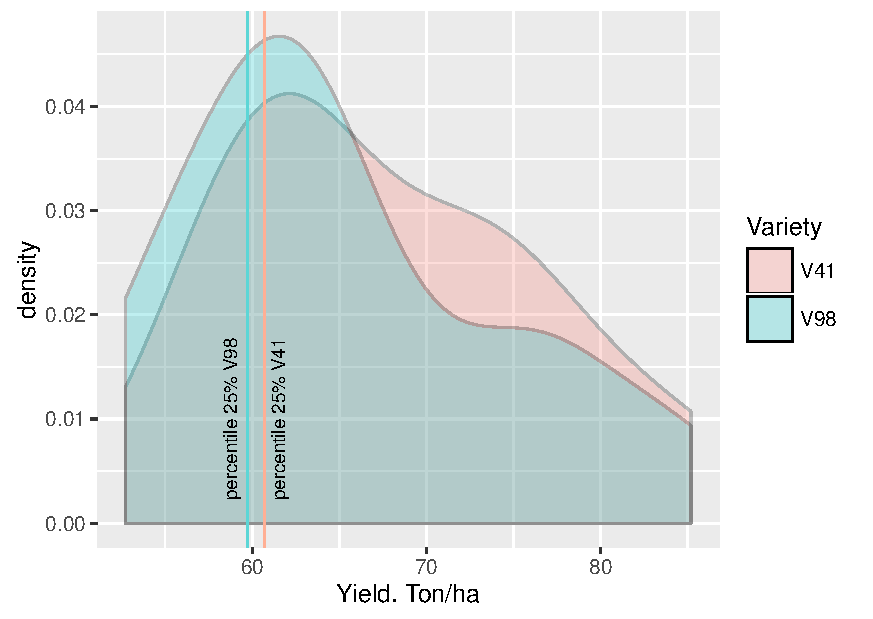
\includegraphics[height=3in]{density2}
\caption{Distribution of Yields for Varieties V41 and V98.} \label{denplot}
\end{center}
\end{figure}

In figure \ref{denplot}, the density distribution of the yield of two relevant varieties -V41 and V98-, in ton.ha\textsuperscript{-1}, is illustrated. 
After pre-processing the data as described in following sections, this graph shows the yields distribution among scenarios, where each scenario -combination of site and season- is considered to have the same probability of occurrence. 
Indubitably, decision makers will prefer those varieties with yield distributions with high mean values and low standard deviations, this last as a measure of the risk. 

\subsection{First quartile as measure of preference}
Alternatively to the mean and standard deviation, an indicator of performance can be expressed in terms of avoiding losses instead of maximizing wins. 
An evaluation metric focused on the left tail of the distribution may be more suitable for the assumption that a robust decision is the one that returns a satisfactory outcome in as many scenarios as possible. 
Therefore, the lower bound of the yield for the 75\% best scenarios, given by the percentile 25\% of the density distribution could be a convenient criteria to asses the convenience of choosing each strategy. 
This metric of risk is widely used in financial markets to estimate how much a set of investments might lose, given normal market conditions. Usually, the threshold value used varies from 1 and 5\%  -\cite {linsmeier2000value}. 
In this study, the percentile value at 25\% is fixed as a criteria, because the same threshold value was set in \cite {lempert2006general}, and also because a small survey conducted by project members among real farmers in Argentina revealed similar preferences when they were asked about their threshold between winning and losing. 
Of the two varieties in the figure \ref{denplot}, V41 would be preferred to V98 as the percentile 25\% value of yield, or first quartile (1Q), is 60.7 vs. 59.7 ton.ha\textsuperscript{-1} respectively.

\subsection{Selecting an initial robust strategy candidate}

The RDM procedure requires the selection of initial robust strategy candidate to continue later exploring its vulnerabilities. 
In a real context, this candidate could be chosen as the strategy recommended by farmer's usual decision method. 
In this study, the strategy -variety or mix of varieties- with the highest value of 1Q is selected as initial candidate. The mix with the given percentages: 50\% of variety 187, 50\% of variety 41 is the strategy with the maximum value of 1Q of yield: 62.62 ton.ha\textsuperscript{-1}.
As a notation, strategies will be referred as X\textsubscript{1}VY\textsubscript{1}\_X\textsubscript{2}VY\textsubscript{2}, where X denotes the proportion of land and Y denotes the variety. 
Hence, the candidate is notated as 0.5V187\_0.5V41. 
Once selected the initial strategy, its performance is explored among the set of scenarios evaluated focusing on identifying vulnerabilities (i.e., characteristics of scenarios where the candidate does not perform acceptable).
In this study, the varieties V41 and V187 will be explored individually. Although, very similar results can be obtained analyzing the performance of strategy 0.5V187\_0.5V41 as a mix. 

\subsection {Identification of vulnerabilities} 

\begin{figure}[t]
\begin{center}
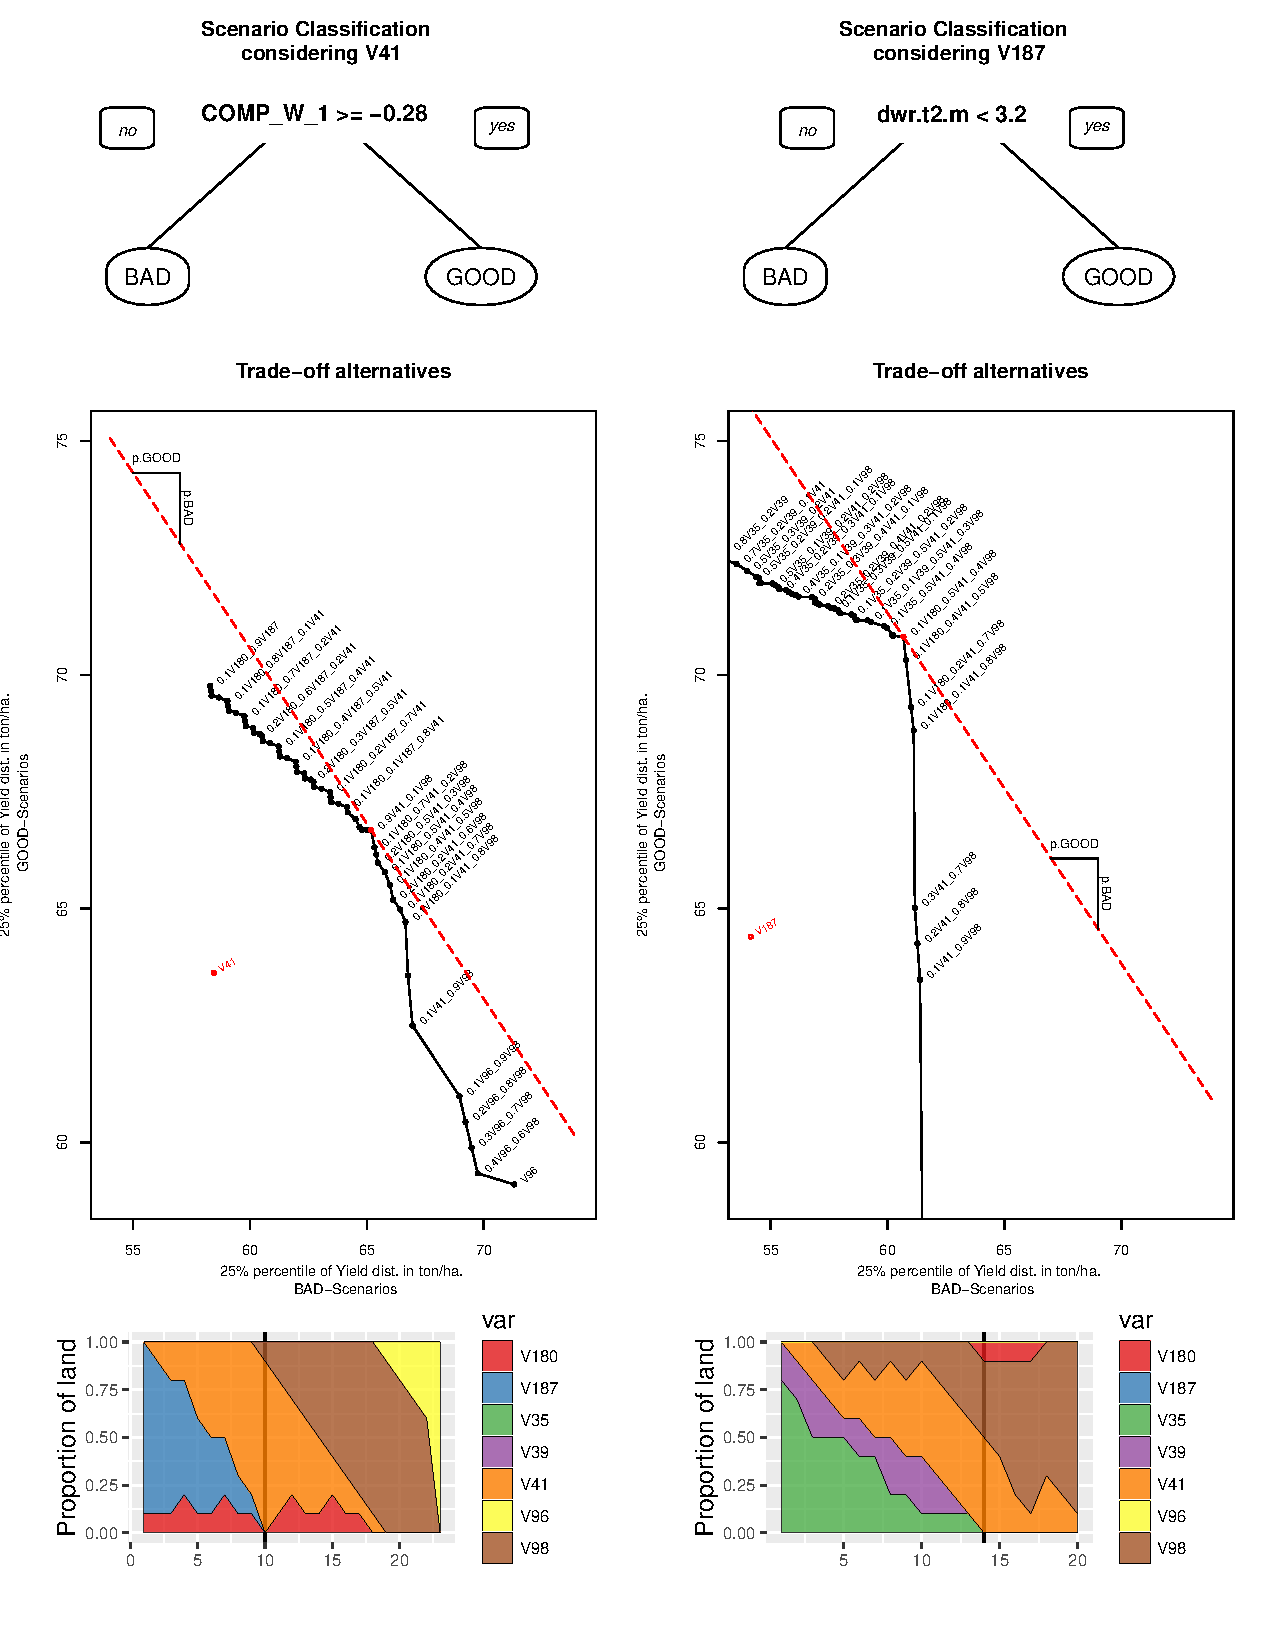
\includegraphics[height=7in]{frontier}
\caption{Selection of variety mix.} \label{frontier}
\end{center}
\end{figure}

The ideal robust strategy would have no vulnerabilities. 
Unfortunately, this is generally not the case. 
This subsection explores the exposure to an unacceptable result of candidates, first V41 and then V187. 
In this regard, the contexts that create unfavorable conditions –and therefore lower outcomes– for these strategies need to be identified. 
This stage is often referred to in the literature as "scenario discovery" -\cite{bryant2010thinking}. 
Various data-mining algorithms can be used to find combinations of parameters that are most strongly predictive of decision-relevant regions in a dataset. 
After a series of operations applied to the data which include aggregation, Clustering, and PCA, this study implements a classification tree algorithm -\cite{breiman1984classification}- to discriminate situations where initial candidate strategy V41 (and V187) has "good" and "bad" performance. 
The usage of classification trees in RDM was explored in \cite{lempert2008comparing}. 
An advantage of the tree approach is that the sets of conditions that lead to a bad performance can be easily interpreted and communicated to decision-makers. 
In the top-left graph in figure \ref{frontier} the tree that classifies the scenarios into "good" or "bad" depending on whether the yield of variety V41 is higher or lower than the 1Q is depicted. 
Each scenario -combination of site and season- is characterized by a series of features related to the soil and aggregated weather, together with principal components calculated. 
Details about the considerations to run the tree and the operations performed is detailed in next section.
The tree obtained has only one split and two leafs and classifies the scenarios according to the value of 1\textsuperscript{st} principal component calculated from the scenario weather data in the PCA analysis. 
If the value of the 1\textsuperscript{st} weather principal component, which is the component that captures most of the variability of the weather data, is lower than -0.28, then the scenario is classified by the tree as "bad".
This component has a close relationship (high absolute value of coefficients) with the variables associated with the average of maximum and minimum temperatures within the period between March the 1\textsuperscript{st} and May the 31\textsuperscript{st}. -see table \ref{pca} for details. 
When analyzing the training data for strategy V41, the scenario discovery stage unveils the pattern followed by scenarios that cause an unsatisfactory result. 
The decision outcome to assign 100\% of land to V41 is jeopardized by scenarios that have a low value of the 1\textsuperscript{st} principal component of weather data. 
Therefore, this classification implies that V41 has poor performance in cold years, mainly between March and June, and variables related to rainfall, soil type, radiation seem to have less impact on the a low performance.

\subsection{Identification of hedging strategies} 

Last section discussed the range of conditions in which initial candidate V41 does not perform well (e.g., when temperatures are low in average). 
This subsection aim to find alternative strategies that provide hedges against scenarios in which strategy V41 is vulnerable.
As a first step, the classification tree grown before is used to classify all scenarios into "good" or "bad" categories. 
That is, the entire set of scenarios is divided into two groups according to the predicted performance of initial candidate V41 in each scenario. 
To explore hedging alternatives, the performances of all strategies for the two subsets of scenarios divided by the classification tree are evaluated.
In one subset, all scenarios will exhibit the value of the 1\textsuperscript{st} principal component of weather data higher than -0.28; those will be labeled as "good".
The other subset will be labeled as "bad" and scenarios there will be identified as their principal component value lower than -0.28. 
For each strategy, the first quartile (1Q) of yield values are calculated considering separately "good" and "bad" scenarios. 
Then, these quartiles are used as coordinates in a plot of a subset of strategies with highest yield values to form a preference frontier similar to a Pareto frontier. -Figure \ref{frontier} in the middle-left.
Initial strategy 0.5V187\_0.5V41 had the highest 1Q in all actual scenarios. 
Note, however, that when calculating 1Q of yield separately for predicted "good" and "bad" scenarios, strategy 0.5V187\_0.5V41 has no longer the highest 1Q. 
Instead, strategy 0.1V180\_0.9V187 shows the highest 1Q for scenarios in which strategy V41 was predicted to have "good" performance; that is, 0.1V180\_0.9V187 is the highest point along the y-axis. 
Similarly, strategy V96 (lower right of figure) has the highest 1Q of yield in "bad" scenarios.
An ideal alternative to strategy V41 would have high values of yield under both "good" and "bad" scenarios. 
Such strategy would be preferred over all other possible land allocations, as it would perform satisfactorily regardless of the scenario that might occur. 
Unfortunately, the figure does not show an ideal strategy −which would be located in the higher right corner of the figure. 
Instead, the values delineate a 'preference frontier' defined by the higher right edge of a cloud of points (i.e., strategies). 
Strategies along the frontier dominate other strategies: for a given yield in "bad" scenarios (x-axis), strategies under the frontier have lower (i.e., worse) yield.

In summary, alternative strategies were identified, all of which have satisfactory performance under a broad range of future states of the world. 
That is, all strategies located along the frontier represent robust alternatives among which a farmer may choose. 
The selection, however, will depend on the decision-maker’s expectations about the future. 
If farmers expect a "bad" scenario (i.e., cold temperatures in March-May), they should chose allocation strategy V96. 
If the opposite conditions are expected, strategy 0.1V180\_0.5V187, at the other end of the frontier, seems the better choice. 
Inevitably, however, choice among strategies involves trade-offs. 
As frontier is traveled from left to right, the yield of strategies decreases for "good" scenarios while increases for "bad" scenarios. 
To select one strategy from the frontier, real decision makers may use their own sources of information to predict how next scenario is going to be. 
Also, their final decision may depend on their own experiences, knowledge, and their risk profile. 
Nevertheless, another way to pick a final decision mix is by computing the odds or the likelihood to happen a "good" or a "bad" scenario, as in \cite {lempert2006general}. 
In this example, daily information in the evaluation dataset is available to compute the first weather principal component for historical years and estimate the probability for the evaluation site to have the weather component greater (or lower) than -0.28. 
In 3 out of 7 years considered (i.e., 2008, 2013 and 2014), the first principal component of weather data in evaluation site determines that the scenario was labeled as "bad", which indicates low average temperatures. 
Therefore, the probability of "bad" can be estimated as p(bad)=0.4285 for the evaluation scenario. 
Consequently, the probability of "good" is p(good)=1-p(bad)=0.5715. 
A red dotted line in the mid-left plot in figure \ref{frontier} represents a line with slope=-p(bad)/p(good). 
This line determines the optimal mix that maximizes the expected value of the 1Q considering the odds for "good" and "bad" scenarios. 
Taking this likelihood into account, decision makers should select the strategy 0.9V41\_0.1V98. 
If farmers expect months between March and May to be a colder than the historical series data -determined by variable COMP\_W\_1-, this methodology suggests they should try strategies with higher percentage of V98 and V96. 
Otherwise (i.e., March-May months expected to be warmer or average), strategies abundant in V187 should better mitigate the risk of a low outcome.

Once an alternative is evaluated, decision-maker could begin again exploring its vulnerabilities and start the same procedure over. 
For example, strategy V96 may be a feasible option when cold weather is expected. 
Also interesting will be to explore the conditions where the assignment of V96 is not a good choice.
An iterative process may be convenient to evaluate many varieties or mix of varieties. 

\subsection {Strategy V187 as an alternative initial candidate}
 
Similarly to V41, the vulnerabilities of variety V187 can be studied by exploring the training data. 
The classification by the tree in the top-right figure \ref{frontier} indicates that this seed seems to have a low yield when the consecutive days without precipitations are, in average, greater than 3.2 within the month of July, August and September. 
This tree recognizes the pattern "bad" scenarios as the years with rainfalls not-well-uniformly distributed. 
Then, the scenarios can be divided again, this time into "good" and "bad" according to the value of the defined variable that measures the consecutive days without rainfalls. 
In the scatter plot in the mid-right figure, alternatives that mitigate the risks when expected a "bad" scenario can be found.
The preference frontier indicates that strategies rich in V98 and V41 should be preferred.
The plot also shows that the trade-offs are not very favorable to the strategies at the very right because the frontier is almost a vertical line. 
The slope in the line suggests that the 1Q value decreases rapidly for "good" scenarios while it does not increase in the same amount for "bad" scenarios. 
Computing the odds of the average of consecutive days in the evaluation site historical data, it can be verified that in years 2009, 2011, and 2013 the average value of days without rainfalls in July-September were higher than 3.2 days, therefore the probability of can be estimated as 3/7, p(bad)=0.4285. 
These odds generate a line that intersects with the frontier in a point that represents strategy 0.1V180\_0.5V41\_0.4V98, which seems to be a good compromise.

In summary, the yield of strategy V187 appears to be sensible to the distribution of rains. 
When expected the historical patter of rains, the odds show that 0.1V180\_0.5V41\_0.4V98 may be a suitable decision. 
When rains are expected to be more uniformly distributed than the historical record, then V35 or V39 may better limit the possibilities of a low yield. 
Unfortunately, when the distribution of precipitations is expected to be less homogeneous, there is no strategy that can reduce the possibility of failure.

In essence, the two explorations of vulnerabilities of V41 and V187 produce similar results. 
They both suggest as a compromise strategies with percentage of these seeds: V41 and V98. 
The strategy recommended in the abstract was calculated as the average of two intersection points -the vertical lines in below stacked plots-. 
Nevertheless, the intention of this methodology is not only to provide a single point as a recommendation, but also to generate relevant knowledge to allow farmers to take better decisions.

\section{Methodology and theory}

This study modeled the decision to select a strategy (i.e., variety or mix of varieties) considering as possible scenario the conjunction of (i) site, with general climate features and soil features, and (ii) season, with daily weather information corresponding to each historical year. 
Given a strategy, the yield obtained will depend on the variables that define each scenario. 
Therefore, a dataset was constructed to implement the methodology correspondingly.
This dataset has the following fields: (i) \texttt{SCENARIO} (Combination of \texttt{SITE} and \texttt{SEASON}) and its variables, (ii) \texttt{VARIETY} or variety mix, and (iii) yield -\texttt{VARIETY\_YI}-, or combined yield when the strategy is a mix, (iv) 22 distinctive features related to the \texttt{SITE}, and (v) 58 features as aggregation of daily weather data linked to the \texttt{SITE}-\texttt{SEASON}, as will be described below. 
This section details an extensive series of steps followed to reach the conclusions presented.

\subsection{Data Pre-processioning}

The file provided \texttt{Training Dataset.xlsx} was the skeleton of the data used for exploration and training of the classification tree. 
First, 2103 records were discarded because they were considered duplicates. 
Then, variables \texttt{CLIMATE} and \texttt{SOIL\_CUBE} were decomposed into 3 numerical variables each and variable \texttt{RM\_BAND} was converted to a numeric variable. 
The missing values in \texttt{CONUS\_PH} were replaced by values obtained as predictions from a linear regression with all other soil features as predictors. 

\subsection{Scenario Data Construction}

The unbalance in the database was an issue because many records with the same pair variety-scenario may lead to a biased conclusions. 
To deal with that, those records were grouped together to generate only one record for each variety-scenario pair. 
As the values of the variables that define a scenario are the same, the median of the yields values in the scenario was assigned to the yield field value in the new record.

\begin{figure}[t]
\begin{center}
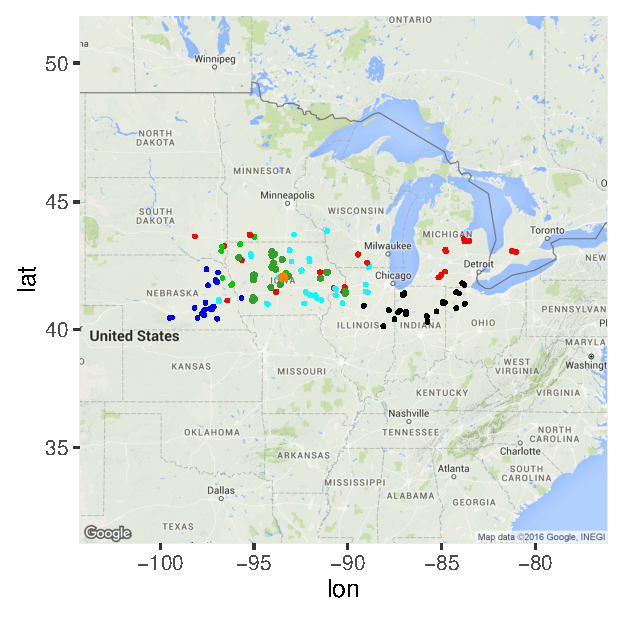
\includegraphics[height=4in]{map1}
\caption{Location of sites considered after clustering (green dots).} \label{map}
\end{center}
\end{figure}

\subsection{Clustering of Sites}

Taking into account that the site data is given in evaluation, to consider only the test records placed in those sites that are very much alike the site provided as evaluation is more accurate to minimize the uncertainty. 
This assumption drives a very cautious approach, as the sites where the actual test occurred have almost identical attributes as the site evaluated, reducing the risk of unexpected result. 
To select those sites, first, a k-means algorithm -\cite{arrow1956berkeley}- was executed to group the sites into clusters with similar characteristics.
Then, only the records in which the weighted euclidean distance between their site and the evaluation site is lower than a threshold were kept for training. 
The weighted distance calculated compares the scaled values not only of Latitude and Longitude, but also the difference between the values of all features related to the site, as, for instance, irrigation and the soil type, etc.
Just in this clustering, the features identifying the site related to climate were excluded, as those variables were considered as uncertain and considered in by the aggregation of daily data.
Either the number of cluster (k) or the threshold distance to identify the closest sites can play a role as parameters to tune the model. 
A higher value of the threshold or a smaller value of k will allow take into account more diverse sites giving more generality to the model.
A map with the location of the sites similar to the evaluation site is showed in figure \ref{map}.
%which includes a K-means clustering  and a Principal Component Analysis 

\subsection{Aggregation of daily data}

The training data to explore the varieties performance is structured in a time frame with yearly aggregation according to the season, from 2008 to 2014. 
Therefore, a series of operations was required to incorporate the daily weather information available to a yearly aggregation. 
First, the entire year was separated into 3 sub periods of time. 
According to \cite {pedersen2004soybean}, the growth and development of soybean is within the 60 first days since the sowing planting date. 
Also, in \cite{spd2006}, the author suggests a optimum time to plant soybean in Iowa at May the 1\textsuperscript{st}. 
Hence, the year daily series is divided as showed in table \ref{stages}.

\begin{table}
\begin{center}
\begin{tabular}{cccc}
\hline
Id    & Start Date & End Date & Description   \\
\hline
t\textsubscript{0}      & 1-Mar    & 30-Apr & Pre-Planting   \\
t\textsubscript{1}      & 1-May    & 30-Jun & Growing and development    \\
t\textsubscript{2}      & 1-Jul    & 30-Sep & Maturity \\
\hline
\end{tabular}
\end{center}
\caption{Times to aggregate the daily data according to stages in soybean crop production.}\label{stages}
\end{table}

The 3 periods of time involve: 60 days of pre-planting climate, 60 days of growing, starting from the planting date 1-May, and 90 days of maturity. 
These periods detailed were used to aggregate all daily data presented in the \texttt{Training daily weather dataset}. 
To aggregate the daily data, a set of functions was applied to the data as described in table \ref{agg}. 
Also, two new daily variables were calculated: \texttt{dwr}, consecutive days without rain, and \texttt{trange}, as the difference between the maximum and minimum temperatures. 

For example, variable \texttt{tmax.t0.mi} is the minimum value of maximum temperature registered in days between 1-May and 30-Jun. 
Also, \texttt{dwr.t2.me} is the average of consecutive days without precipitation records in days between the months of July and September. 
As discussed in previous section, the value of this variable has a significant importance to identify scenarios in which variety V187 returns a poor yield.

\begin{table}
\begin{center}
\begin{tabular}{lclc}
\hline
Variable   & name & function & provided/calculated   \\
\hline

Day length	& \texttt{dayl }& mean & provided\\
Precipitation & \texttt{prcp} & mean & provided \\
Consecutive days without \texttt{rain} & dwr & mean, max & calculated \\
Shortwave radiation	&\texttt{srad} & mean, max, min& provided\\
Snow water equivalent	& \texttt{swe} & mean, max& provided\\
Maximum air temperature	& \texttt{tmax} & mean, max, min& provided\\
Minimum air temperature	& \texttt{tmin} & mean, max, min& provided\\
Temperature range (tmax-tmin) & \texttt{trange}& mean, max, min & calculated\\
Water vapor pressure	&\texttt{vp }& mean, max& provided\\
\hline
\end{tabular}
\end{center}
\caption{Variables generated and functions applied to aggregate daily weather.}\label{agg}
\end{table}

\subsection{Principal components analysis}
% 2 paragraph (overview + explanation)

Besides dimension reduction, another application of principal component analysis -\cite{hotelling1933analysis}- is to data pre-processing. 
In this case, the goal is not to deal with multiple features but rather to transform the data set in order to allow subsequent pattern recognition algorithms to be applied successfully. -\cite{bishop2006pattern}.
This study applied PCA to generate the projections to permit the classification tree to categorize the observations accurately. 
After defining the new variables and aggregating the daily data, the features were divided into two groups: features related to the site, and features related to the climate conditions. 
PCA was applied to the scaled dataset considering each subset of features separately.
The components generated were appended as new columns to the training dataset; 20 components related to the site and 58 components related to the weather data. 

\begin{table}
\begin{center}
\begin{tabular}{lrr}
\hline
Variable   & \texttt{COMP\_W\_1} & \texttt{COMP\_W\_2}   \\
\hline

\texttt{prcp.t0.me}  & &  0.200\\
\texttt{prcp.t1.me}  & & 0.184\\
\texttt{prcp.t2.me}  &  &-0.223\\
\texttt{tmax.t0.me}  &  0.225 &\\
\texttt{tmax.t1.me}  &  0.230 &\\
\texttt{tmax.t2.me} &  0.189&  \\
\texttt{tmax.t1.ma}  &  & 0.213\\
\texttt{tmax.t2.ma}  &   &0.209\\
\texttt{tmax.t0.mi}  & &  0.212\\
\texttt{tmax.t2.mi}  &  & 0.250\\
\texttt{tmin.t0.me}  &  0.233 &\\
\texttt{tmin.t1.me}  &  0.211&  \\
\texttt{tmin.t0.ma } &   &-0.184\\
\texttt{tmin.t0.mi } &  &  0.210\\
\texttt{trange.t0.me} & & -0.194\\
\texttt{trange.t2.me}  &0.196  & \\
\texttt{trange.t0.mi}&  &-0.218\\
\texttt{vp.t0.me   }  & 0.221 &\\
\texttt{vp.t1.me}    &  0.189 & \\

\hline
\end{tabular}
\end{center}
\caption{Coefficients of the two first principal components of weather data. \newline Only coefficients with absolute values higher than 0.18 are showed.}\label{pca}
\end{table}

The table \ref{pca} shows the highest coefficients, in absolute value, to calculate the first and second components given the values or the variables. 
The first principal component, in any PCA, is the one that captures most of the variability of the data.
Therefore, the coefficients of the fist component indicate that the variability of the weather information is defined primarily by the average of maximum and minimum temperatures. 
Also, the value of the first component \texttt{COMP\_W\_1} was the main driver to identify scenarios that leads to a poor performance of variety V41. 
The second component, showed just for illustration, has relation with the range of temperatures, rather that their average values, and with the level of rainfalls. 
The original features, plus the defined variables, plus the 78 principal components appended, plus the keys: variety and scenario, generate a dataset used to train the supervised algorithm.
This dataset contains each variety individually.
To consider mix of varieties as possible strategies new records need to be generated.

\subsection {Strategy generation as variety combination}
% 1 paragraph

To generate possible strategies as a mix of varieties, new test cases were created. 
Given a particular scenario -combination of site and season-, more than one variety could be tested. In that case, a strategy consisting in a mix of those varieties can be produced. 
The scenario data can be copied straightforward, the strategy receives a name according to the mix (i.e., 0.5V41\_0.5V98), and the yield of the mix is calculated as a linear combination of the yields of each variety. 
For simplicity, only increments of 10\% were considered to define the mix in the land assignment and a maximum of 5 different varieties to be assigned to a land.

\subsection {Classification tree}

Once performed the operations previously described, the training dataset is ready to evaluate the varieties and all the variety mixes generated. 
To start the exploration, the methodology begins with a candidate. 
In this study, V41 and V187 were analyzed. 
Starting from V41, scenarios can be labeled depending whether the value of the yield of this strategy is lower or higher than its first quartile (i.e., lower than 60.7 ton.ha\textsuperscript{-1})
Labeling manually the scenarios into "good" and "bad", a categorical target variable can be defined to permit the using of a classification tree to recognize which are the patterns that leads to a "bad" performance. 
The tree algorithm will explore all the feature space with more than 150 features describing the land and the weather and discover what are the patterns that have those scenarios labeled as bad. 
The resulting trees are depicted in the top-left tree in figure \ref{frontier} (top-right for V187).
The set of parameter values used to run the algorithm and the simplicity of the tree -only one split with two leafs guarantee that the overfiting is avoided. 

\section{Supplementary materials}

The script implemented was coded in R. 
Some relevant packages used were: \texttt{rpart}, to fit the classification tree -\cite{therneau2015package}; \texttt{cluster}, to implement the k-means cluster analysis -\cite{maechler2015package}; \texttt{ggmap}, to trace the site colored map -\cite{kahle2013ggmap}. 

A full version of the script that implements this study can be downloaded at \url{https://github.com/xavierign/Syngenta}.

%\theendnotes

% Acknowledgments here
\ACKNOWLEDGMENT{This research was supported by Argentina National Agency for Scientific and Technological Promotion, grant ANPCyT PICT 2014-1344 \textit{'Big Data in agriculture decision-making'}, the Peruilh fellowship of the School of Engineering at the University of Buenos Aires and the 'Argentine Presidential Fellowship in Science \& Technology'.}

\bibliographystyle{ormsv080}
\bibliography{mypaper.bib} % if more than one, comma separated

%%%%%%%%%%%%%%%%%
\end{document}
%%%%%%%%%%%%%%%%%

%%%%%%%%%%%%%%%%%
%TO DO NEXT
%%%%%%%%%%%%%%%%%

% explain the paper to be written
% compare with expected utility
% explain that traditional methods should not be discarded.
% improve the graph


%\begin{itemize}
%\item Supplementary File One Name: file one description
%\item Supplementary File Two Name: file two description 
%\end{itemize}

% intro
%Example of the and figures, such as  Figure, should be used. For pagination reasons, figures and tables may appear on different pages as does Figure   Remember,  the entries will be evaluated based on the following criteria: (1) the rigor and validity of the process used to determine your seed variety recommendation, (2) the quality of the proposed solution, which will be assessed by the alignment with historically observed variety responses at the Evaluation Farm (which are not part of the data distributed to researchers). and (3) additional criteria including (a) simplicity of your solution, (b) the evaluation of factors included in the decision process, and (c) clarity in the explanation.  It is vital that you document your methodology in sufficient detail for evaluation. 

% Present the methodology and theory of your approach.  Charts, diagrams, flowcharts or other visualizations may be useful to communicate your thinking. Including discussion and considerations, such as the assumptions that were made, the scope, and early considerations,  may provide a useful framing of your solution.  Given the multi-disciplinary aspect of the problem,  background information may be useful to include or reference.  It is vital that you document your methodology in sufficient detail and clarity that it can be understood and evaluated. 
% 

 % In this section, you should list the criteria you used to select the seed varieties.  As noted in the Challenge statement, there is substantial interplay between the genetic content of the soybean variety and the changes in environment. In general, there is no seed variety that stands out above the others in all environments. Selecting varieties involves a combination of seeking the best yield and hedging against uncertain environments at the Evaluation Farm (e.g., weather).  The decision to use a variety may also be impacted by the risk profile of the farmer (e.g., gain maximization, loss avoidance). The risk profile can be considered as a factor to propose alternative soybean variety portfolios for the Evaluation Farm.
